\documentclass[../main.tex]{subfiles}

%preamble
% \usepackage[subpreambles=true]{standalone}
% \usepackage{import}
% \usepackage{amsmath}%insert math equation
% \usepackage{graphicx} %insert picture
% \usepackage{subcaption}%insert pictures at the same place
% \usepackage{hyperref}%hyperlink
% \usepackage[a4paper]{geometry}
% \usepackage[section]{placeins}

% \title{Aspheric Surface Derivation}
% \date{2018-02-02}
% \author{Hongjie Lu}

\begin{document}

	% \maketitle
	% \pagenumbering{gobble}
	% \newpage
	\section{Spheric}
	\begin{figure}[h!]
	  \centering
	  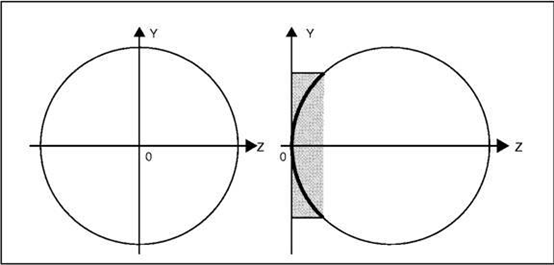
\includegraphics[scale=0.7]{../graphics/aspheric_1.png}
	  \caption{Coordinate translation}
	  \label{fig:sag}
	\end{figure}
	Figure \ref{fig:sag} shows the coordinate translation to the left vertex of the surface. The math equations before and after the coordinate translation are as follows:
	\begin{align}
		z^2 + y^2 &= R^2\\
		z^2 - 2zR + y^2 &= 0\\
		Pz^2 - 2zR + y^2 &= 0
	\end{align}
	where $P = 1 + K$, and $K = -e^2$. e is the eccentricity with $e^2 = \frac{a^2 - b^2}{a^2}$, a is the major axis for the conic section and b is the minor axis.
	For the left half part we are interested in,
	\begin{align}
		z &= \frac{R-\sqrt{R^2-Py^2}}{P}\\
		z &= \left(\frac{R}{P}\right)\left[1-\sqrt{1-P\left(\frac{y}{R}\right)^2}\right]\\
		z &= \frac{cy^2}{1+\sqrt{1-(1+K)c^2y^2}}
	\end{align}
	\begin{figure}[h!]
		\centering
		\begin{subfigure}[b]{0.5\linewidth}
			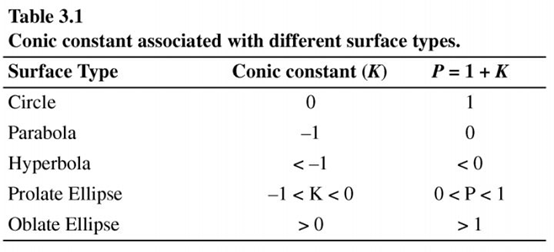
\includegraphics[width=\linewidth]{../graphics/aspheric_2.png}
			\caption{Conic constant}
		\end{subfigure}
		\begin{subfigure}[b]{0.3\linewidth}
			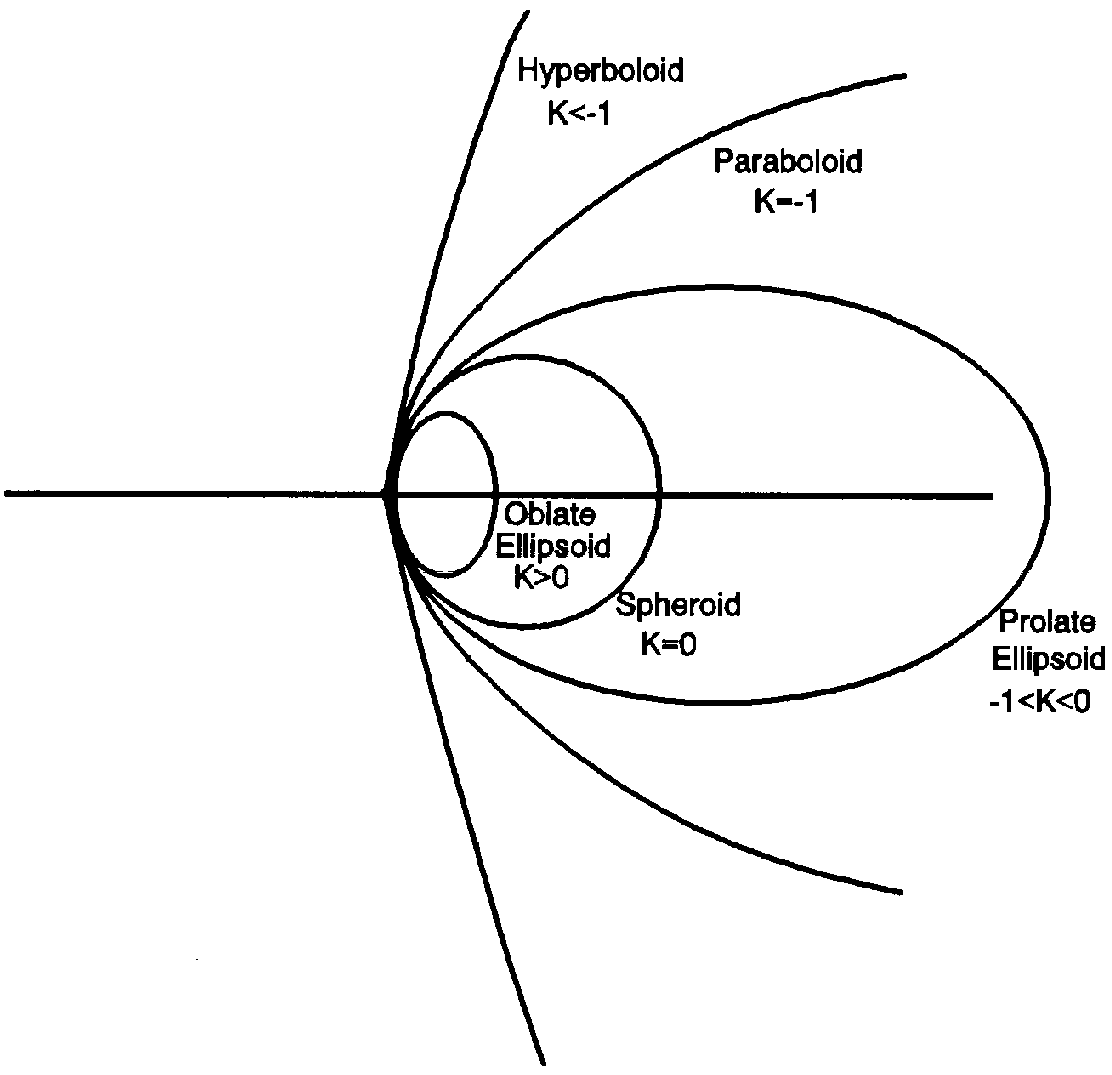
\includegraphics[width=\linewidth]{../graphics/aspheric_3.png}
			\caption{Relative shapes of conic surfaces in two dimensions}
		\end{subfigure}
		\caption{Conic surfaces}
	  	\label{fig:conic_constant}	  
	\end{figure}
	We call z the sag of the surface -- the displacement from the vertex, K is the conic constant, c is the surface curvature and y is the radial height on the surface.
	We can get different conic section surface types when we choose different K values.

	Conic mirrors give perfect geometric imagery when an axial point object is located at one conic focus and the axial point image is located at the other conic foucs.
	\begin{figure}[h!]
	  \centering
	  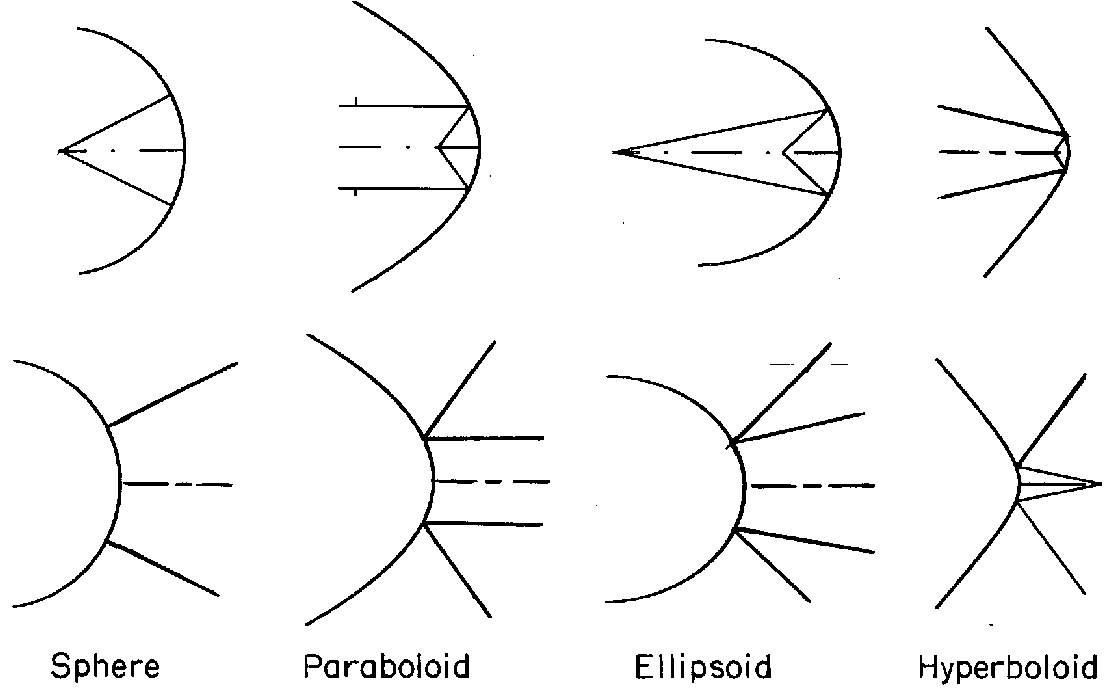
\includegraphics[scale=0.5]{../graphics/aspheric_4.png}
	  \caption{Ray paths for perfect axial imagery}
	  \label{fig:conic_ray}
	\end{figure}

	\section{Aspheric}
	General aspheres are surfaces with fourth- and higher-order surface deformation on top of a flat or curved surface. The surface deformation of a rotationally sy,,etric general asphere is given by the relation
	\begin{equation}
		z = \frac{cy^2}{1+\sqrt{1-(1+K)c^2y^2}}+Ay^4+By^6+Cy^8+Dy^10
	\end{equation}
	where A,B,C and D are 4th-, 6th-, 8th-, and 10th=order coeffcients that determine the sign and magnitude of the deformation produced by that order. Although general aspheres allow correction of third- and higher-order aberrations and may reduce the number of elements in an optical system, general aspheres are more expensive than spheres or conics. If aspheric deformation is required, conic surfaces should be tried first, especially since a conic offers higher-order correction.

	\section{Reference:}
	\url{https://zhuanlan.zhihu.com/p/29930116}\\
	Handbook of Optics, Chapter 18
\end{document}